%%%%%%%%%%%%%%%%%%%%%%%%%%%%%%%%%%%%%%%%%
% Programming/Coding Assignment
% LaTeX Template
%
% This template has been downloaded from:
% http://www.latextemplates.com
%
% Original author:
% Ted Pavlic (http://www.tedpavlic.com)
%
% Note:
% The \lipsum[#] commands throughout this template generate dummy text
% to fill the template out. These commands should all be removed when 
% writing assignment content.
%
% This template uses a Perl script as an example snippet of code, most other
% languages are also usable. Configure them in the "CODE INCLUSION 
% CONFIGURATION" section.
%
%%%%%%%%%%%%%%%%%%%%%%%%%%%%%%%%%%%%%%%%%

%----------------------------------------------------------------------------------------
%	PACKAGES AND OTHER DOCUMENT CONFIGURATIONS
%----------------------------------------------------------------------------------------

\documentclass{article}

\usepackage{fancyhdr} % Required for custom headers
\usepackage{lastpage} % Required to determine the last page for the footer
\usepackage{extramarks} % Required for headers and footers
\usepackage[usenames,dvipsnames]{color} % Required for custom colors
\usepackage{graphicx} % Required to insert images
\usepackage{listings} % Required for insertion of code
\usepackage{courier} % Required for the courier font
\usepackage{lipsum} % Used for inserting dummy 'Lorem ipsum' text into the template
\usepackage{hyperref}
\usepackage{minted}

% Margins
\topmargin=-0.45in
\evensidemargin=0in
\oddsidemargin=0in
\textwidth=6.5in
\textheight=9.0in
\headsep=0.25in

\linespread{1.1} % Line spacing

% Set up the header and footer
\pagestyle{fancy}
\lhead{} % Top left header
\chead{\hmwkClass: \hmwkTitle} % Top center head
\rhead{\firstxmark} % Top right header
\lfoot{\lastxmark} % Bottom left footer
\cfoot{} % Bottom center footer
\rfoot{Page\ \thepage\ of\ \protect\pageref{LastPage}} % Bottom right footer
\renewcommand\headrulewidth{0.4pt} % Size of the header rule
\renewcommand\footrulewidth{0.4pt} % Size of the footer rule

\setlength\parindent{0pt} % Removes all indentation from paragraphs

%----------------------------------------------------------------------------------------
%	NAME AND CLASS SECTION
%----------------------------------------------------------------------------------------

\newcommand{\hmwkTitle}{DBMS Project} % Assignment title
\newcommand{\hmwkClass}{Data Modeling and Databases} % Course/class
%\newcommand{\hmwkClassTime}{10:30am} % Class/lecture time
\newcommand{\hmwkClassInstructor}{Qiang Qu} % Teacher/lecturer
\newcommand{\hmwkAuthorName}{Alexey Chernyshov, Vladislav Kravchenko, Murad Magomedov} % Your names

%----------------------------------------------------------------------------------------
%	TITLE PAGE
%----------------------------------------------------------------------------------------

\title{
\vspace{2in}
\textmd{\textbf{\hmwkClass:\ \hmwkTitle}}\\
\vspace{0.1in}\large{\textit{\hmwkClassInstructor\ }}
\vspace{3in}
}

\author{\textbf{\hmwkAuthorName}}
\date{} % Insert date here if you want it to appear below your name

%----------------------------------------------------------------------------------------

\begin{document}

\maketitle

%----------------------------------------------------------------------------------------
%	TABLE OF CONTENTS
%----------------------------------------------------------------------------------------

%\setcounter{tocdepth}{1} % Uncomment this line if you don't want subsections listed in the ToC

\newpage
\tableofcontents
\newpage

%----------------------------------------------------------------------------------------
\section{Phase 1. Design and Implement Relational Model.}

\subsection{Introducing}
There are many repositories containing research article information, but not all of them provide interfaces to access this information. Thus we decided to use DBLP. One of its interfaces is (https://aminer.org/billboard/citation), which provides such additional information as cites and abstracts for articles. This information further will be used in ranking methods. 

\subsection{ER-Model}
After studying the documentation we agreed on next entities for our ER-model: 
\begin{itemize} 
	\item Article
	\item Author
	\item Keyword
\end{itemize} 
We will extract Keywords from the abstracts in order to search for related articles.
We designed this ER-Model:
\newline
\begin{figure}[h!]
  \centering
      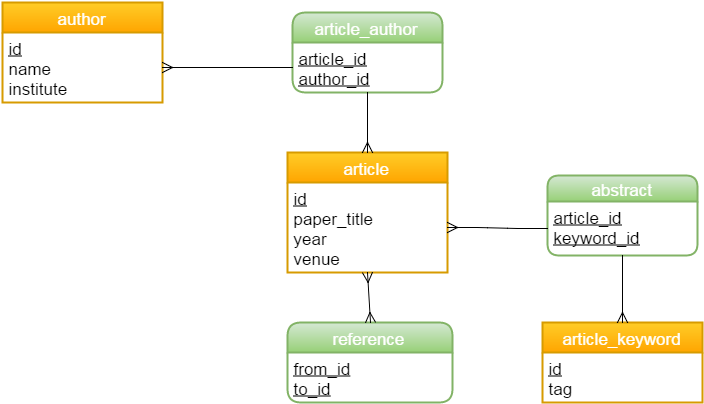
\includegraphics[width=1\textwidth]{ER.png}
  \caption{ER-Model diagram.}
\end{figure}

\newpage
Our ER-Model was transformed into Relations:
\begin{itemize} 
	\item article: \{[\underline{id: INTEGER}, paper\_title: STRING, venue: STRING, year: INTEGER]\}
	\item author: \{[\underline{id: INTEGER}, name: STRING, institute: STRING]\}
	\item keyword: \{[\underline{id: INTEGER}, tag: STRING]\}
	\item article\_author: \{[\underline{id\_article: INTEGER}, \underline{id\_author: INTEGER}]\}
	\item article\_keword: \{[\underline{id\_article: INTEGER}, \underline{id\_keyword: INTEGER}]\}
	\item reference: \{[\underline{from\_id: INTEGER}, \underline{to\_id: INTEGER}]\}
\end{itemize} 

\subsection{Functionality}
We designed the relations in an existing database management system (DBMS) by creating physical tables and their relationships. For our DBMS we have chosen the PostgreSQL. We imported 1.632.442 publications that we parsed using a Python script from an existing publication repository (DBLP).
In addition, we created the SQL-query files that perform such operations:
\begin{itemize} 
	\item Select
	\item Update
	\item Delete
	\item Insert
\end{itemize}
You can search the publication based on author name, publication year, venue(conference/journal name), title, keyword, institution. 

To search for the related articles you can use Keywords and References (to\\from).

You can sort the publications based on such ranking methods:
\begin{itemize} 
	\item based on the number of times the Authors were cited. (In case of a new publication with no references to, but with popular authors)
	\item based on the number of times the Article was cited. (Popular publications)
\end{itemize}
SQL-query files can be found in attachment.
\\


\newpage
\section{Phase 2. Web-based User Interface.}

\subsection{Introducing}
According to Project Phase2 requirements we had to develop a web-based graphical user interface on top of physical database that we had created at Phase 1. \\
After considering different high-level programming languages we decided to use Python because of its clean, straightforward syntax and great support for building web apps. And as it was suggested by instructors on piazza.com we used PostgreSQL for the database management system and Tornado web framework for the web-based GUI.

\subsection{Setup Instructions}

1. Install Python: https://www.python.org/download/releases/3.4.0/ \\
2. Install PostgreSQL: http://www.postgresql.org/download/ \\
3. Import dump: execute in cmd in folder: 
\begin{verbatim}
".../PostgreSQL/9.4/bin/ psql -U 'input your database username here' -f \end{verbatim}
\begin{verbatim}
'path to dump file' 'name of your database' 
\end{verbatim} 
4. Execute query to add auth table:
\begin{verbatim}
...\src\sql\auth\create_auth.sql
\end{verbatim} 
5. Configure Settings.py - set your username and password \\
6. Install Tornado: execute in cmd in folder
\begin{verbatim}
C:\Python34\Lib\site-packages\easy_install.py tornado 
\end{verbatim}
7. Run in cmd webserver.py 
8. Go to http://localhost:8000 \\

\subsection{Functionality}
According to the Phase 2 requirements only authorized/registered users are allowed to use the interface that we have created. The table with usernames and passwords can be stored in another database but in our case we decided to store it at the main database, even it is not logically connected with it.
Authorized/registered users can carry out all the specified functionality, including search, insert (add), update () and delete.
All the search results can be ranged in ascending or descending order.

\newpage
\subsection{Site map}
~
\newline
\begin{figure}[h!]
  \centering
      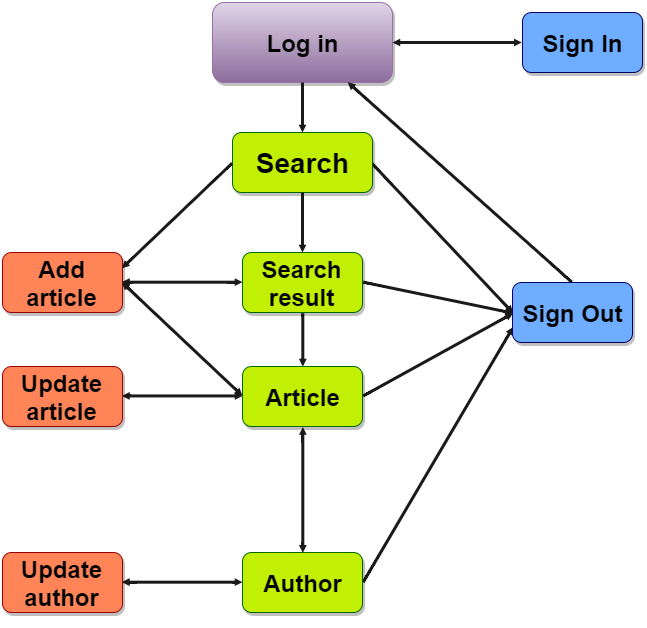
\includegraphics[height=11cm]{sitemap.png}
  \caption{Site Map}
\end{figure}

\newpage
\subsection{Snapshots of the Interface}
~
~
\begin{figure}[h!]
  \centering
      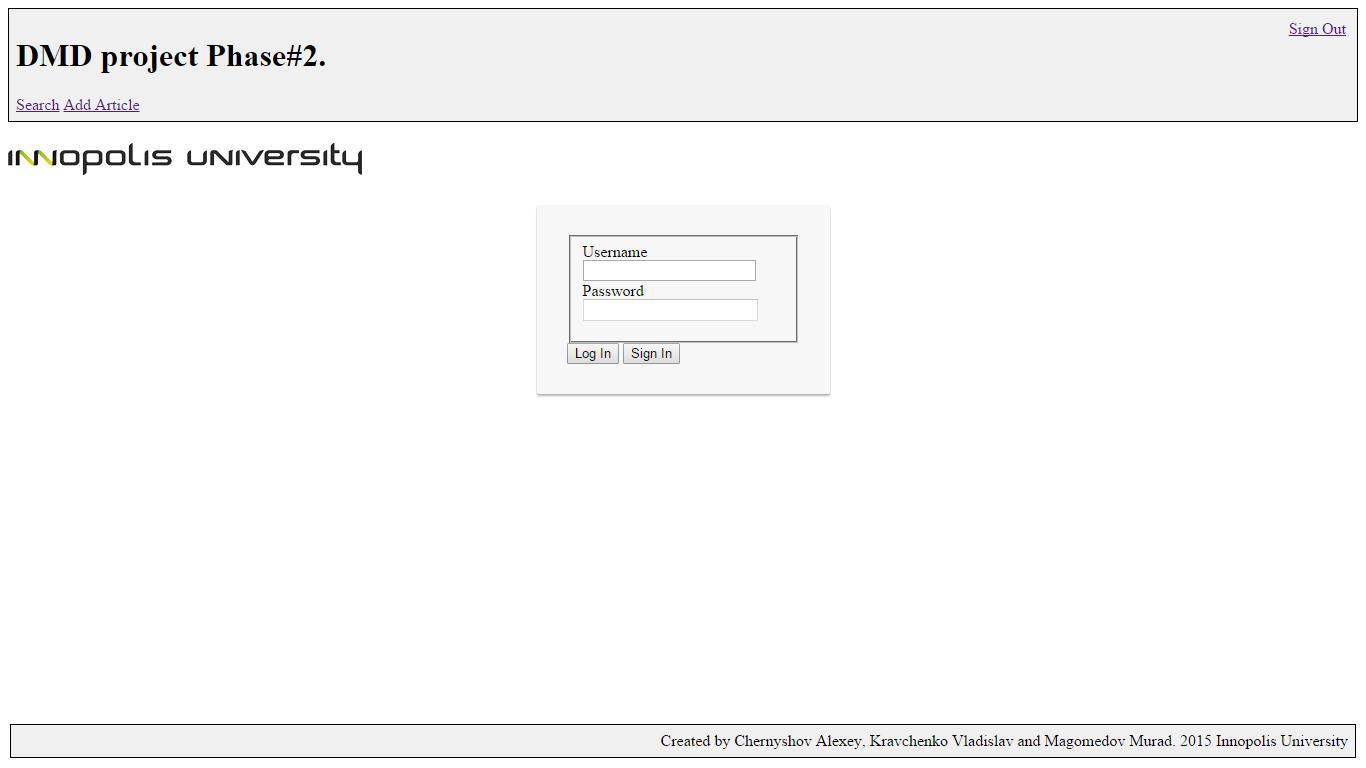
\includegraphics[width=16cm]{1.jpg}
  \caption{Log in or Sign in}
\end{figure}
~
~
\begin{figure}[h!]
  \centering
      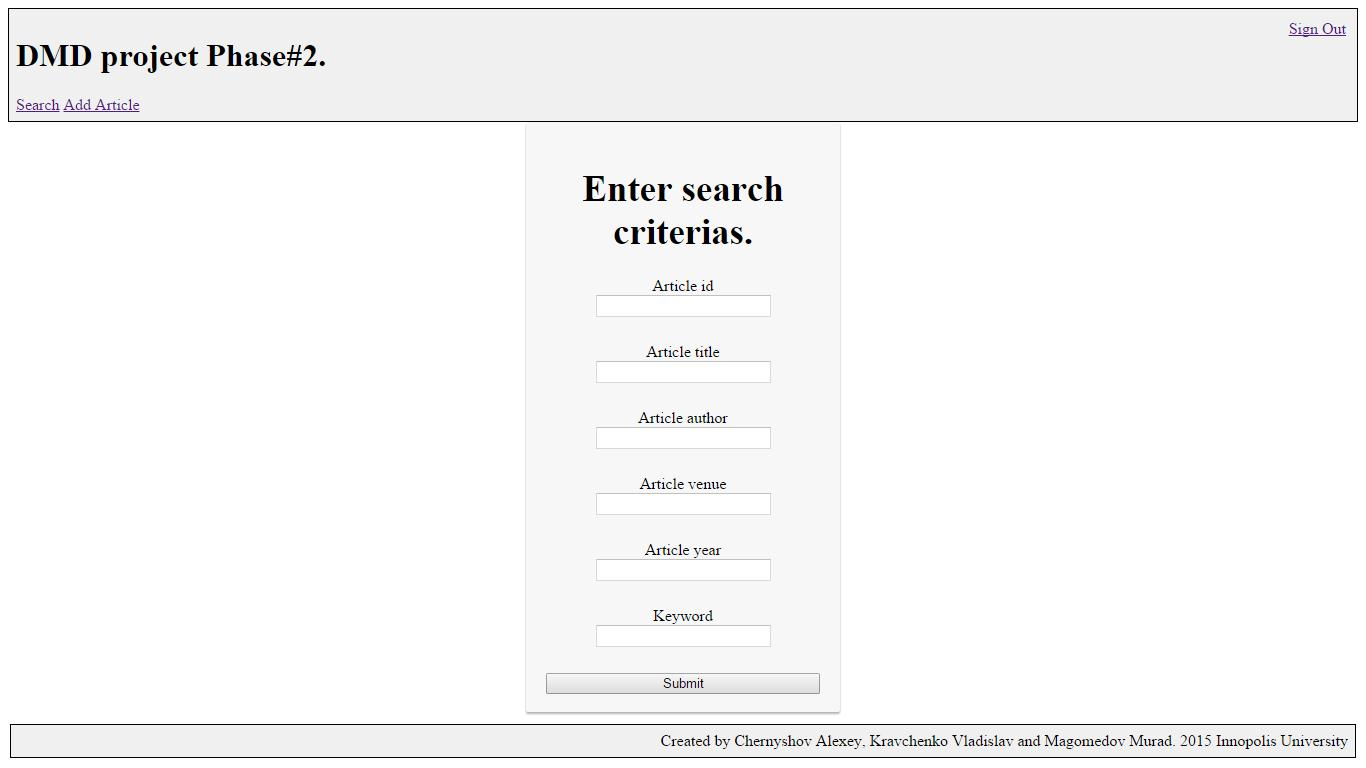
\includegraphics[width=16cm]{2.jpg}
  \caption{Search}
\end{figure}
~
~
\begin{figure}[h!]
  \centering
      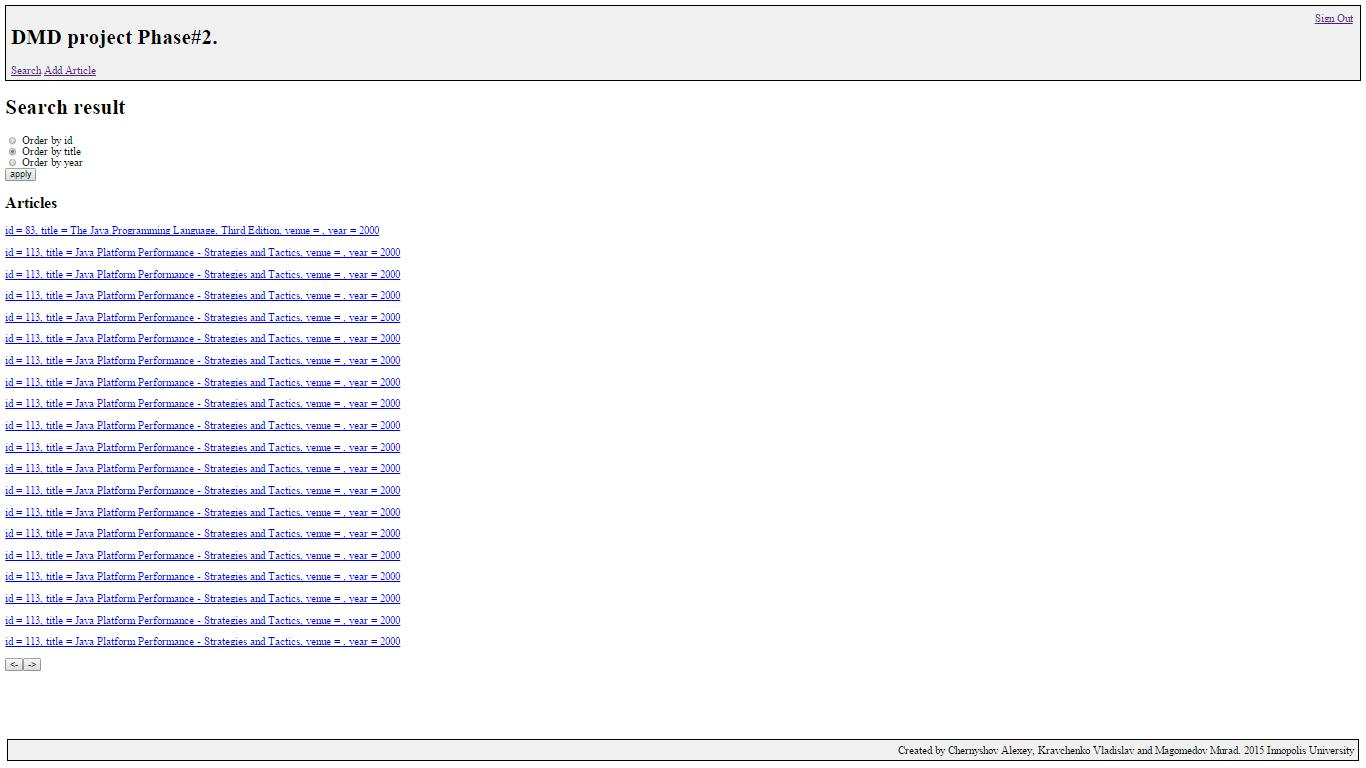
\includegraphics[width=16cm]{3.jpg}
  \caption{Search result}
\end{figure}
~
~
\begin{figure}[h!]
  \centering
      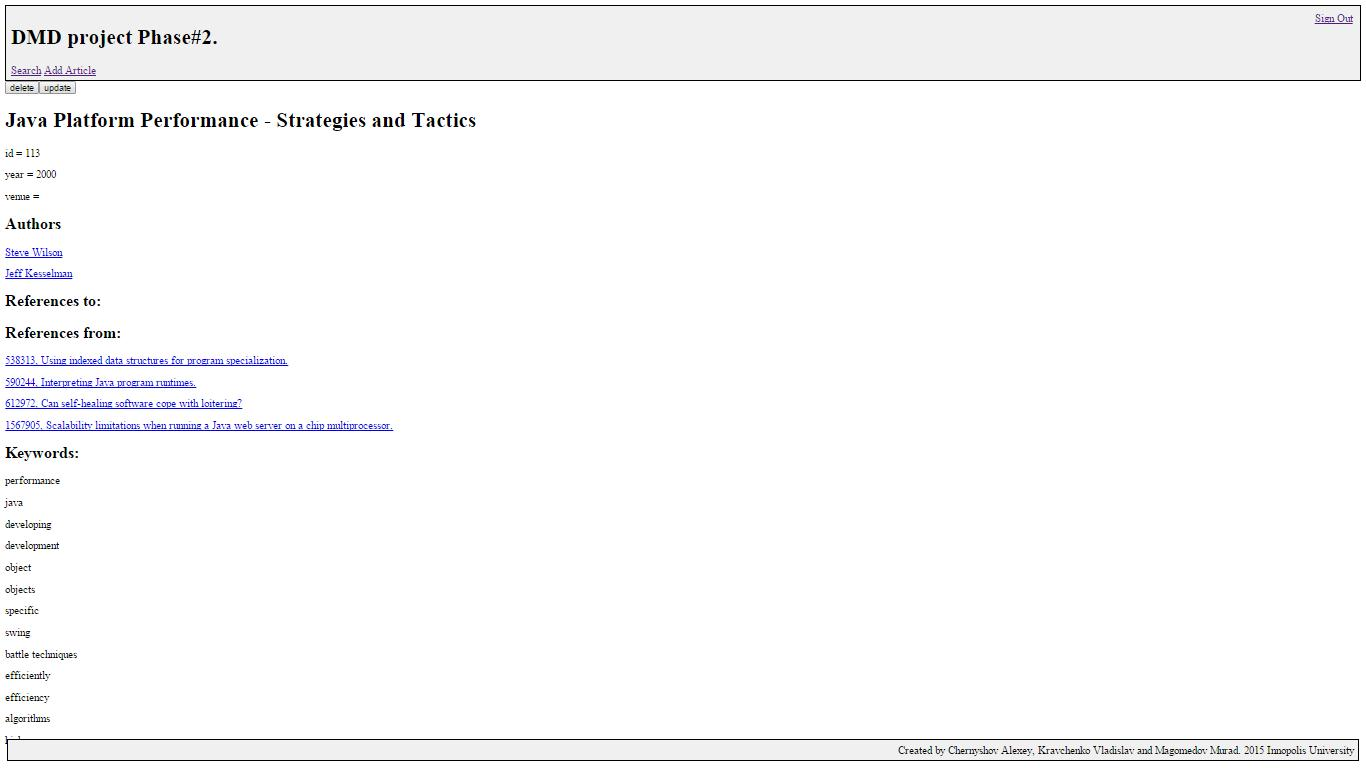
\includegraphics[width=16cm]{4.jpg}
  \caption{Article}
\end{figure}

~

\section{Phase 3. DBMS}

\subsection{Introducing}
According to the Project Phase 3 requirements we had to replace the relational database with our own implementation of a database. We have done it, including the implementation of query operators using python programming language.

\subsection{Setup Instructions}

1. You need to have everything installed from the Phase 2.
2. Run src/dbms/psqlloader.py to create a datafile for your dbms and to import data from Postgres.
3. Configure src/webapp/Settings.py (login, password, database file name)
4. Run web application src/webapp/webserver.py (SQL replaced application)
All SQL was moved to src/webappsql.
5. Go to the http://localhost:8000

\subsection{Functionality}
At the Phase 3 all the SQL code was replaced with calls to the query operators. So now our database provides methods to query data, to insert new records, update existing records and delete them. \\

\textbf{For example, SQL code of Select:}

\begin{minted}{sql}
cur.execute("""SELECT id, name, institute FROM author WHERE id=%s;""", (id, ))
\end{minted}

\textbf{Replaced with:}

\begin{minted}{python}
qr_author = qp.getFromTable('author', )
qr_res = qp.getFromTable('author', ('id', id))
qr_res = qr_res.project('id', 'name', 'institute')
qr_res = qr_res.sort('id')
\end{minted}
~
\\
\textbf{Delete:}

\begin{minted}{sql}
cur.execute("""DELETE FROM article_author WHERE author_id=%s""", (id, ))
\end{minted}

\textbf{Replaced with:}

\begin{minted}{python}
qp.deleteFromTable('article_author', ('author_id', author_id))
\end{minted}
~
\\
\textbf{Update:}

\begin{minted}{sql}
cur.execute("""UPDATE author SET id=%s, name=%s, institute=%s
            WHERE id=%s""", (id, name, institute, id))
\end{minted}

\textbf{Replaced with:}

\begin{minted}{python}
qp.deleteFromTable('author', ('id', id))
qp.addToTable('author', ('id', id), ('name', name), ('institute', institute))
\end{minted}
~
\\
\textbf{Insert:}
\begin{minted}{sql}
cur.execute("""INSERT INTO reference (from_id, to_id)
            VALUES (%s, %s)""", (id, article_id))
\end{minted}

\textbf{Replaced with:}

\begin{minted}{python}
qp.addToTable('reference', ('from_id', id), ('to_id', article_id))
\end{minted}
~
\\
\\
\textbf{Group by:}

\begin{minted}{python}
qres.groupBy('id', 'name')
\end{minted}

\begin{verbatim}
Our database also answers queries that join two tables, for example join of tables 
article_author and article:
\end{verbatim}

\textbf{Join:}

\begin{minted}{python}
qr_article_author = qp.getFromTable('article_author', ('author_id', author_id))
qr_article = qp.getFromTable('article')
qr_res = qr_article_author.join(qr_article, 'article_id', 'id')
qr_res = qr_res.project('article_id', 'paper_title')
qr_res = qr_res.sort('article_id')
\end{minted}

One of the requirements of the Phase 3 was to use the iterator model to implement query operators, so that operators should pull tuples from underlying operators using next() calls. \\
In our case, class qres (query result) is iterable. It is possible to use qres.next or next(qres) to iterate through the results.
In our DBMS it is possible to index on Primary keys with an option to add index on other attributes. \\
And according to Project limitations we are using a single file for the entire DBMS. The Database file is created using psqlloader.py that imports data from Postgres.

\newpage
\subsection{Disk Page Organisation}
~
\newline
\begin{figure}[h!]
  \centering
      \includegraphics[width=17cm]{dpo.png}
  \caption{Disk Page Organisation}
\end{figure}

\newpage
\subsection{Application architecture}
~
~
\begin{figure}[h!]
  \centering
      \includegraphics[width=17cm]{cd.png}
  \caption{Application architecture}
\end{figure}
~
\\
We use an unclustered file - there is no reason to arrange the data entries since it is too expensive to maintain order. To order data use B+ Tree indexes.
Buffer manager is the top level of file I/O that optimises the Query processor and Disk interaction.

~
\\

\newpage
\subsection{Insights}

During the fulfilling of this Project we have implemented the knowledge acquired during the Data Modeling and Databases Course. We have touched the web development (Tornado framework), Python programming language. We organized our cooperation using the Git Hub source code management system. And we all gained some great team work experience.



\newpage
\begin{thebibliography}{1}

\bibitem{def_dblp} 
\url{http://dblp.uni-trier.de/} DBLP

\bibitem{def_aminer} 
\url{https://aminer.org/billboard/citation} aminer.org

\bibitem{def_aminer} 
\url{http://dblp.uni-trier.de/faq/dblpxml[1].pdf} DBLP — Some Lessons Learned by Michael Ley

\bibitem{def_aminer} 
\url{http://dblp.uni-trier.de/xml/docu/dblpxmlreq.pdf} DBLP XML Requests


\bibitem{def_dblp} 
\url{https://www.python.org/} Python v.3.4

\bibitem{def_tornado} 
\url{http://www.tornadoweb.org} Tornado v.4.2.1

\bibitem{def_tornadobook} 
\ Introduction to Tornado. O’Reilly Media, Inc., 2012. \ ISBN: 978-1-449-30907-7

\bibitem{def_postgresql}
\url{http://www.postgresql.org/} Postgresql v.9.4.5

\bibitem{def_psycopg} 
\url{https://pypi.python.org/pypi/psycopg2} Psycopg2 v.2.6.1



\bibitem{def_tornadobook} 
\ Concepts of Database Management. Philip J. Pratt, Joseph J. Adamski. Cengage Learning, 2008. \\ ISBN: 1-4239-0147-9

\bibitem{def_tornadobook} 
\ Database management systems. Raghu Ramakrishnan, Johannes Gehrke. McGraw-Hill., 2003. \\ ISBN: 0-07-246563-8-ISBN 0-07-115110-9 (ISE)

\bibitem{def_tornadobook} 
\ A First Course in Database Systems. Jeffrey D. Ullman, Jennifer Widom. Pearson Education., 2008. \\ ISBN: 978-0-13-502176-7






\end{thebibliography}

\end{document}